\chapter{Theoretical foundation}
\label{cha:theoretical_foundation}
The introduction discussed different applications of rigid fiber simulations. It especially stressed the importance of being able to simulate a large number of fibers in order to generate the various patterns found in real world experiments.

In this chapter, we will present the theoretical foundation of the physics and the mathematical model the simulations are based on. This is required to be able to understand the numerical method used throughout the rest of the thesis. However, the model is only presented in a reduced summary, and for more details please refer to Tornberg and Gustavsson,~\cite{Tornberg2006}.

\section{Stokes flow}
\label{sec:stokes_flow}

We are interested in modeling the behavior of objects immersed in an incompressible fluid. We restrict ourselves to rigid bodies, which are slowly sedimenting in the fluid due to gravity. In the most general case, the flow can be modeled by the Navier-Stokes equations,
\begin{equation}
  \label{eq:naviar_stokes_equations}
  \begin{aligned}
    \rho\left(\frac{\delta \mathbf{u}}{\delta t} + (\mathbf{u} \cdot \nabla)\mathbf{u}\right) &= -\nabla p + \mu\nabla^2\mathbf{u} + \mathbf{f} \\
    \nabla \cdot \mathbf{u} &= 0 \text{.}
  \end{aligned}
\end{equation}
where $\mathbf{u}(\mathbf{x})$ denotes the velocity field, $p(\mathbf{x})$ the pressure field and $\mathbf{f}(\mathbf{x})$ the force acting on the fluid at the location $\mathbf{x} = (x,y,z) \in \mathbb{R}^3$. The constant $\mu$ is the viscosity of the fluid. Solving these equations is quite challenging due to their time dependence and non-linearity. However, in this work we are only concerned with slowly moving objects and the Reynolds number $Re = \frac{\rho U L}{\mu}$ is assumed to be very small. Given the constraint that $Re \ll 1$, the inertial and acceleration terms in the Navier-Stokes Eqns.~\eqref{eq:naviar_stokes_equations} can be neglected and we arrive at the linear and time independent Stokes equations,
\begin{equation}
  \label{eq:stokes_equations}
  \begin{aligned}
    \nabla p - \mu \Delta \mathbf{u} &= \mathbf{f} \quad &\text{in} \quad \Omega \text{,}\\
    \nabla \cdot \mathbf{u} &= 0 \quad &\text{in} \quad \Omega \text{.}
  \end{aligned}
\end{equation}

In addition to these equations we need two boundary conditions to solve the system. The first boundary condition accounts for the influence on the fluid from the presence of the objects. Hence, we force the fluid velocity at the boundary of the object to be equal to the velocity of the object itself. These no-slip conditions on the surface of the objects are defined as
\begin{equation}
  \label{eq:boundary_condition_surface}
  \mathbf{u} = \mathbf{u}_\Gamma  \quad \text{on} \quad  \Gamma \text{,}
\end{equation}
where $\Gamma$ denotes the union of all object surfaces and $\mathbf{u}_\Gamma$ the corresponding surface velocity, thus constraining the fluid to have zero velocity relative to the object surfaces.

The second boundary condition models the fact that the fluid velocity far from the object is not affected by its presence. This is modeled by stating that the velocity field should be equal to a background velocity $\mathbf{U}_0$ at infinity
\begin{equation}
  \label{eq:boundary_condition_background}
  \mathbf{u} \rightarrow \mathbf{U}_0 \quad \text{as} \quad ||\mathbf{u}|| \rightarrow \infty \text{.}
\end{equation}

In our simulations this background velocity is always set to $0$. Through the motion of the immersed objects and the no-slip boundary conditions defined in Eqn.~\eqref{eq:boundary_condition_surface} the dependency on time is reintroduced to the time independent Stokes Eqns.~\eqref{eq:stokes_equations}.

\section{Boundary integral formulation}
\label{sec:boundary_integral_formulation}

The Stokes equations are linear in both velocity and pressure, which allows them to be solved using a number of different methods for linear partial differential equations. The approach used in this thesis is the boundary integral method, e.g. Pozrikidis,~\cite{Pozrikidis1992}.

\subsection{Fundamental solutions}
\label{subsec:fundamental_solutions}

We start from a boundary integral formulation of the Stokes equations, for which analytical solutions can be derived, so-called fundamental solutions. One such solution is the Stokeslet. If $\mathbf{f}$ in Eqn.~\eqref{eq:stokes_equations} is given by a point force acting at $\mathbf{y}$ with strength $\mathbf{F}$, i.e. $\mathbf{f} = \mathbf{F} \cdot \delta(\mathbf{x} - \mathbf{y})$, where $\delta(\mathbf{x} - \mathbf{y})$ is the Dirac delta function, the velocity field
\begin{equation}
  \label{eq:stokeslet_velocity_field}
  u_i(\mathbf{x}) = \frac{1}{8\pi\mu}S_{ij}(\mathbf{x},\mathbf{y})F_j \quad i,j=1,2,3 \text{,}
\end{equation}
where the tensor product
\begin{equation}
  \label{eq:stokeslet_tensor_product}
  S_{ij}F_j = S_{i1}F_1 + S_{i2}F_2 + S_{i3}F_3 \text{,}
\end{equation}
is a solution to the Stokes equations. The term $S_{ij}$ is the Stokeslet and is given by
\begin{equation}
  \label{eq:stokeslet_stokeslet}
  S_{ij}(\mathbf{x} - \mathbf{y}) = \frac{\delta_{ij}}{|\mathbf{x}-\mathbf{y}|} + \frac{(x_i - y_i)(x_j-y_j)}{|\mathbf{x}-\mathbf{y}|^3}\text{.}
\end{equation}

Later, we will need higher order fundamental solutions to the Stokes Eqns.~\eqref{eq:stokes_equations}. These can be obtained by simply differentiating the Stokeslet. One example is the so-called doublet
\begin{equation}
  \label{eq:doublet}
  D_{ij}(\DIFFPOINT) = \frac{1}{2} \Delta S_{ij}(\DIFFPOINT) = \frac{1}{8\pi\mu} \left( \frac{\mathbf{I}}{|\DIFFPOINT|^3} - \frac{3((x_i - y_i)(x_j-y_j))^2}{|\DIFFPOINT|^5}\right) \text{.}
\end{equation}

\subsection{Formulation for objects immersed in a fluid}
\label{subsec:formulation_objects_in_fluid}

Using the fundamental solution from Eqn.~\eqref{eq:stokeslet_velocity_field} we can now model the influence of immersed objects on the Stokes flow. Assume that we have a total of $M$ immersed rigid objects in the fluid. Each object $m$, for $m = 1,2,\dots,M$ is centered at $\POS_c^m$ with an associated orthonormal basis $\ORIENT^m$ and surface $\Gamma^m$. Given a rigid body motion and the no-slip boundary condition from Eqn.~\eqref{eq:boundary_condition_surface} we can model the velocity field $\mathbf{u}(\POS)$ at each surface point $\POS \in \Gamma^m$ of the object as
\begin{equation}
  \label{eq:rigid_body_motion}
	\mathbf{u}(\mathbf{x}) = \mathbf{U}^m + \mathbf{\omega}^m \times (\POS - \POS_c^m) \text{,}
\end{equation}
where $\mathbf{U}^m$ is the translational velocity of the object and $\mathbf{\omega}^m$ the rotational velocity. This setup is illustrated for $M=2$ fibers in Fig.~\ref{fig:immersed_rigid}.

\begin{figure}[!htbp]
  \centering
  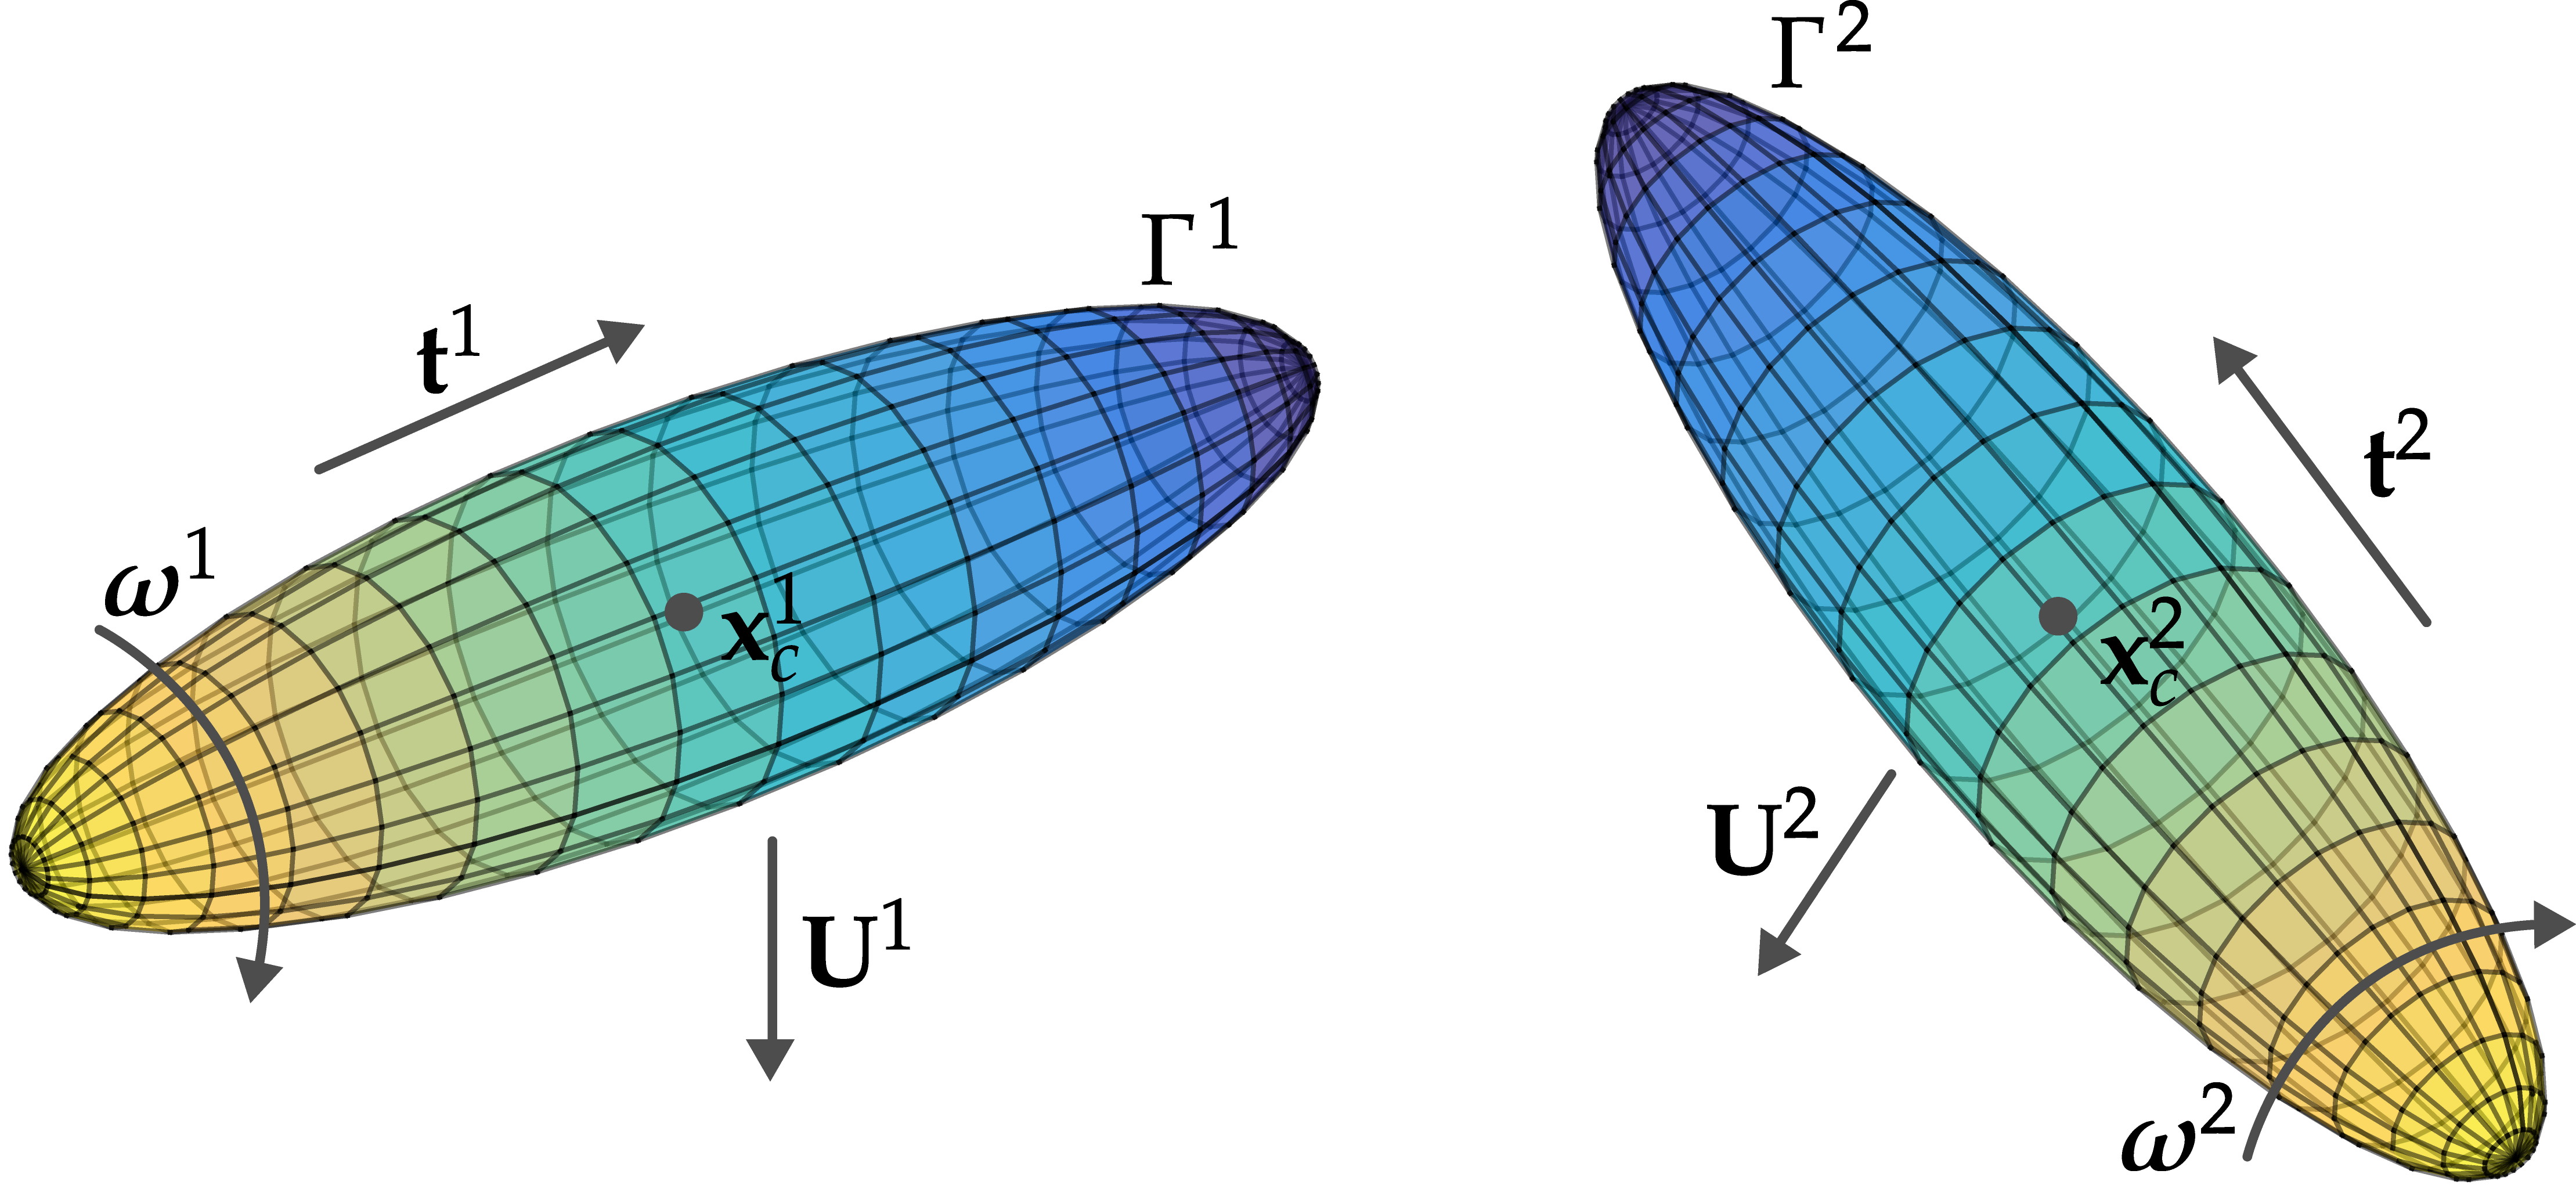
\includegraphics[width=.8\textwidth]{img/immersed_rigid.png}
  \caption[Two immersed objects in stokes flow.]{Two immersed objects in stokes flow, using a rigid body motion. Each fiber is characterized by the positions $\POS^1, \POS^2$ and the orientations $\ORIENT^1,\ORIENT^2$. The velocity of each point the surfaces $\Gamma^1, \Gamma^2$ is given by the rigid body motion described in Eqn~\eqref{eq:rigid_body_motion}.}
  \label{fig:immersed_rigid}
\end{figure}

By combining the rigid body motion with the boundary integral formulation in Eqn.~\eqref{eq:stokeslet_velocity_field} of the Stokes equations we can now relate the objects velocities with the force exerted by all other objects. For this we take advantage of the linearity of the Stokes equation and apply the superposition principle. The superposition principle states that the combined effect from all objects at a single point in the flow is simply the sum of all the individual effects caused by each object. For $M$ fibers this yields the following relationship between the objects velocities and the force distribution , $f$, on the surface of the object,
\begin{equation}
  \label{eq:objects_boundary}
	\mathbf{U}_i^m + (\mathbf{\omega}^m \times (\POS - \POS_c^m))_i = \frac{1}{8 \pi \mu} \sum_{l=1}^{M} \int_{\Gamma^l} S_{ij}(\mathbf{x},\mathbf{y})f_j^l(\mathbf{y}) \, dS_y \quad i,j =1,2,3 \text{.}
\end{equation}

For a sedimenting object, the translational and rotational velocities $\mathbf{U}^m$ and $\mathbf{\omega}^m$ as well as the force distribution $\mathbf{f}^m$ are unknown. Thus in order to be able to solve the system we add two constraints
\begin{equation}
	\label{eq:objects_boundary_constraints}
	\mathbf{F}_{\text{object}}^m = \int_{\Gamma^m} \mathbf{f}^m(\mathbf{y}) \, dS_y\text{,} \quad \mathbf{T}_{\text{object}}^m = \int_{\Gamma^m} (\POS - \POS_c^m) \times \mathbf{f}^m(\mathbf{y}) \, dS_y \text{,}
\end{equation}
stating that the integrated force and torque over each object must be equal to the externally applied force and torque on the object. Given these additional constraints we are now able to solve Eqns.~\eqref{eq:objects_boundary} and~\eqref{eq:objects_boundary_constraints} for $\mathbf{f}^m$, $\mathbf{U}^m$ and $\mathbf{\omega}^m$ for all fibers $m=1,2,\dots,M$. Using the resulting velocities we can then update the position and orthonormal basis of each object through time $t$ by
\begin{equation}
	\label{eq:objects_update}
	\frac{d}{dt}\POS_c^m = \mathbf{U}^m \text{,} \quad \frac{d}{dt}\ORIENT^m = \ORIENT^m \times \mathbf{\omega}^m \text{.}
\end{equation}

Additionally, given the force distribution $\mathbf{f}_m$ of each fiber we can compute the velocity field $\mathbf{u}_i(\mathbf{x})$ at any point $\POS$ in the domain of interest of the Stokes flow. We again take advantage of the superposition principle and apply it to Eqn.~\eqref{eq:stokeslet_velocity_field} to express the velocity field as
\begin{equation}
	\label{eq:objects_velocity_field}
	\mathbf{u}_i(\mathbf{x}) = \frac{1}{8 \pi \mu} \sum_{l=1}^M \int_{\Gamma^l} S_{ij}(\mathbf{x},\mathbf{y})\mathbf{f}_j^l(\mathbf{y}) \, dS_y\text{.}
\end{equation}
The integral appearing in the right-hand side of Eqn.~\eqref{eq:objects_boundary} must in most cases be evaluated by numerical quadrature.

\section{Slender fibers}
\label{sec:slender_fibers}

The formulation developed in the previous section is now adapted for a particular rigid fiber suspension. Consider a straight, rigid body of length $2L$ and radius $a$, and let $\epsilon = a / 2 L$ denote a slenderness parameter. If $\epsilon \ll 1$ the body is referred to as a slender body (slender fiber) as illustrated in Fig.~\ref{fig:slenderness}.

\begin{figure}[!htbp]
  \centering
  \begin{subfigure}[h]{0.24\textwidth}
    \centering
    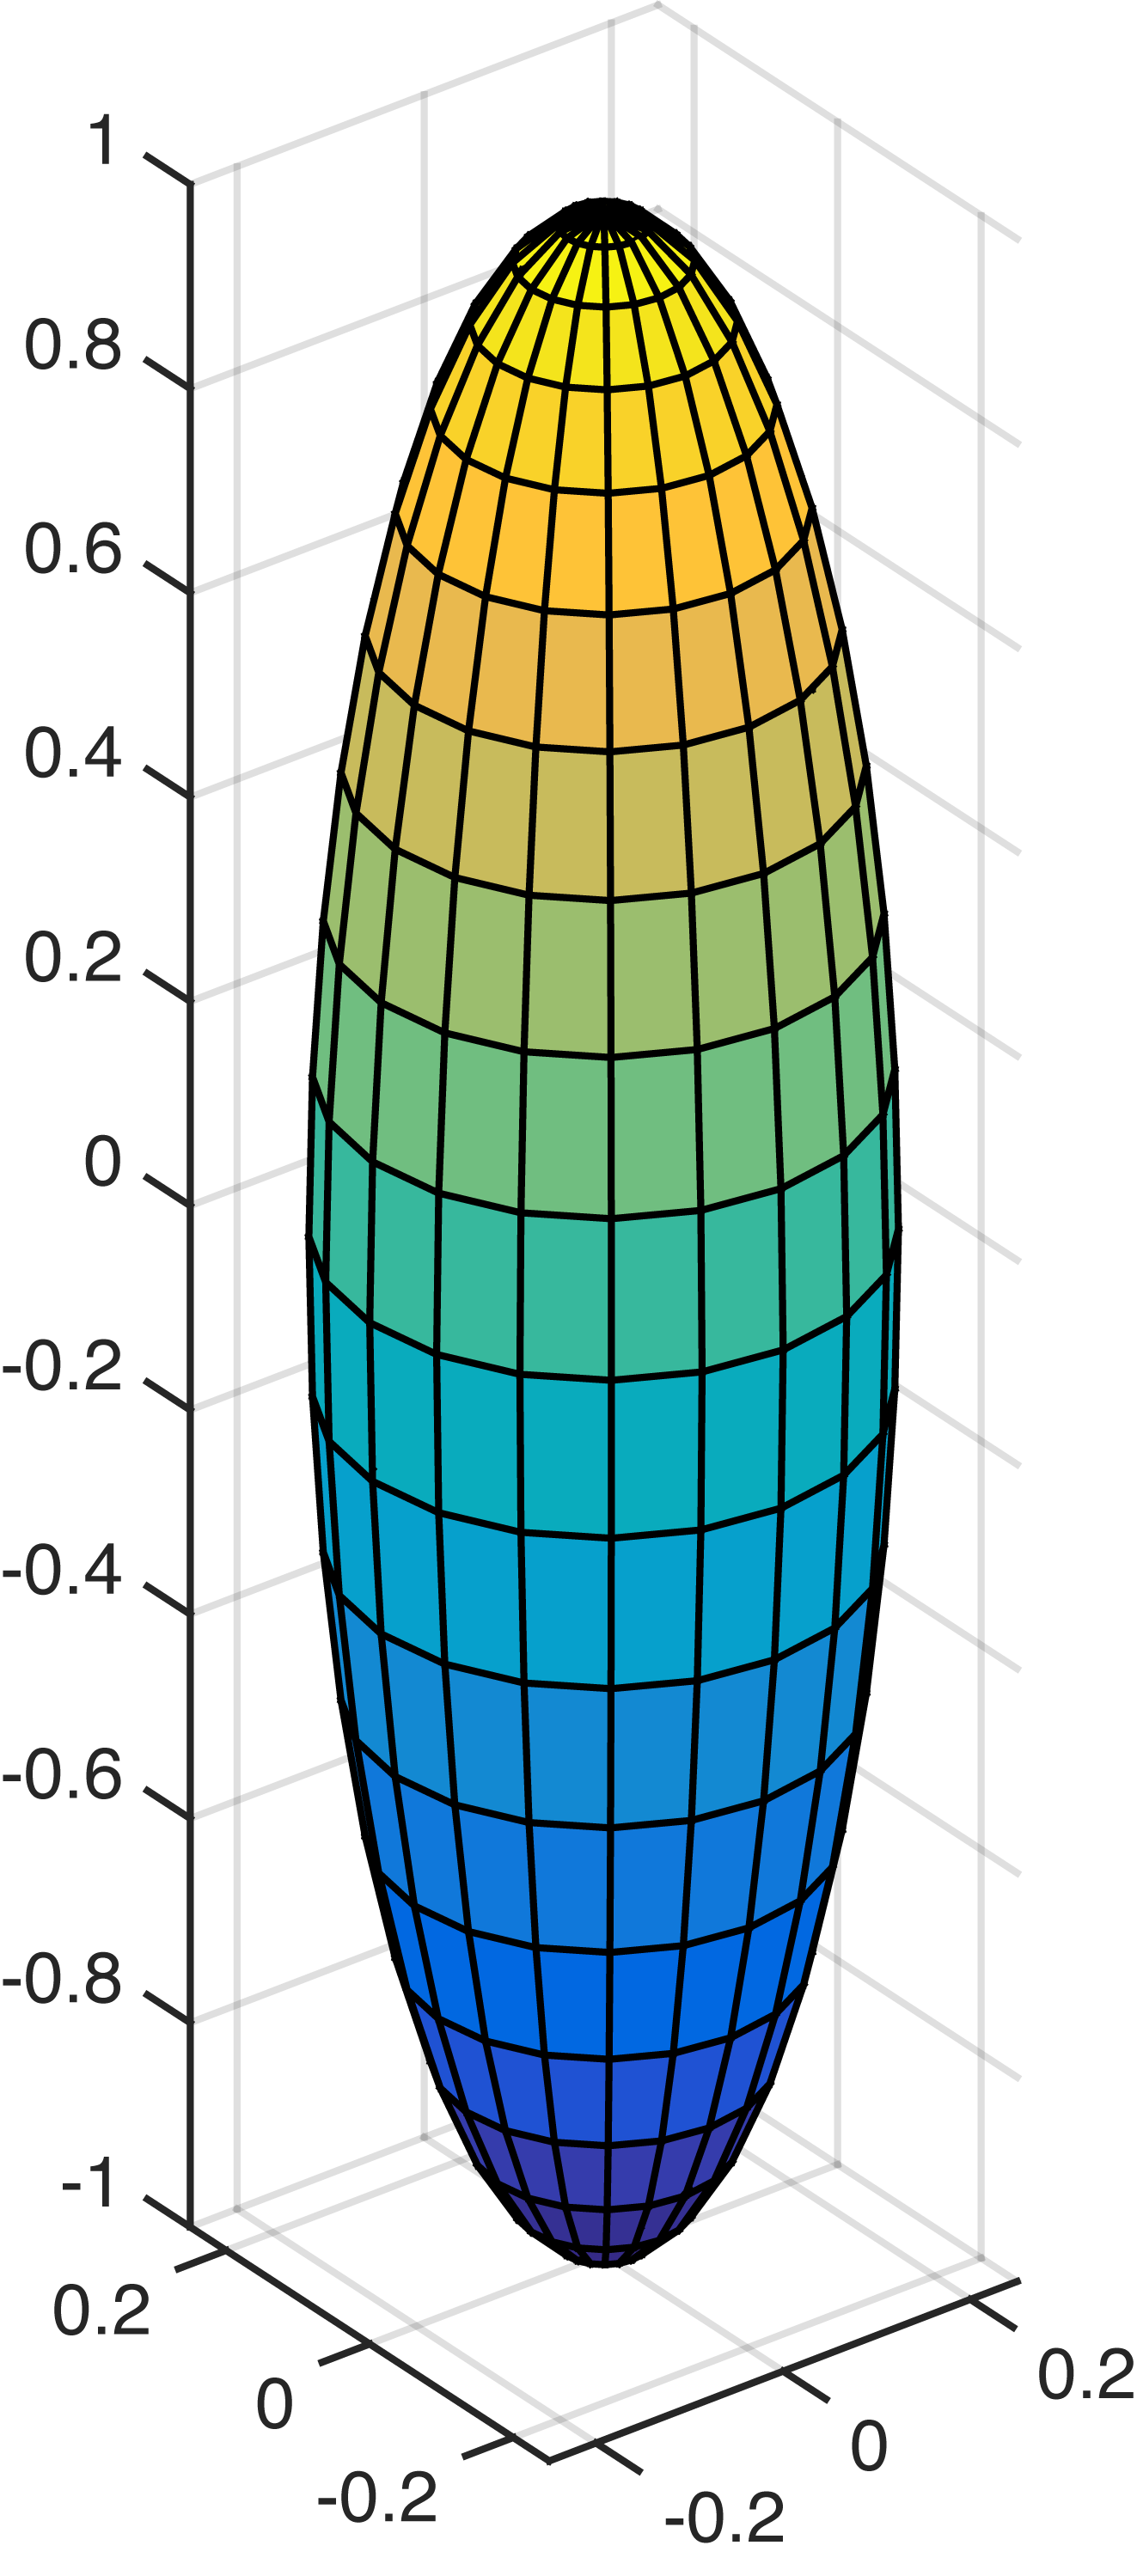
\includegraphics[width=\textwidth]{img/slender/1_4.png}
    \caption{$\epsilon=1/4$}\label{fig:slenderness_1_4}
  \end{subfigure}
  \begin{subfigure}[h]{0.24\textwidth}
    \centering
    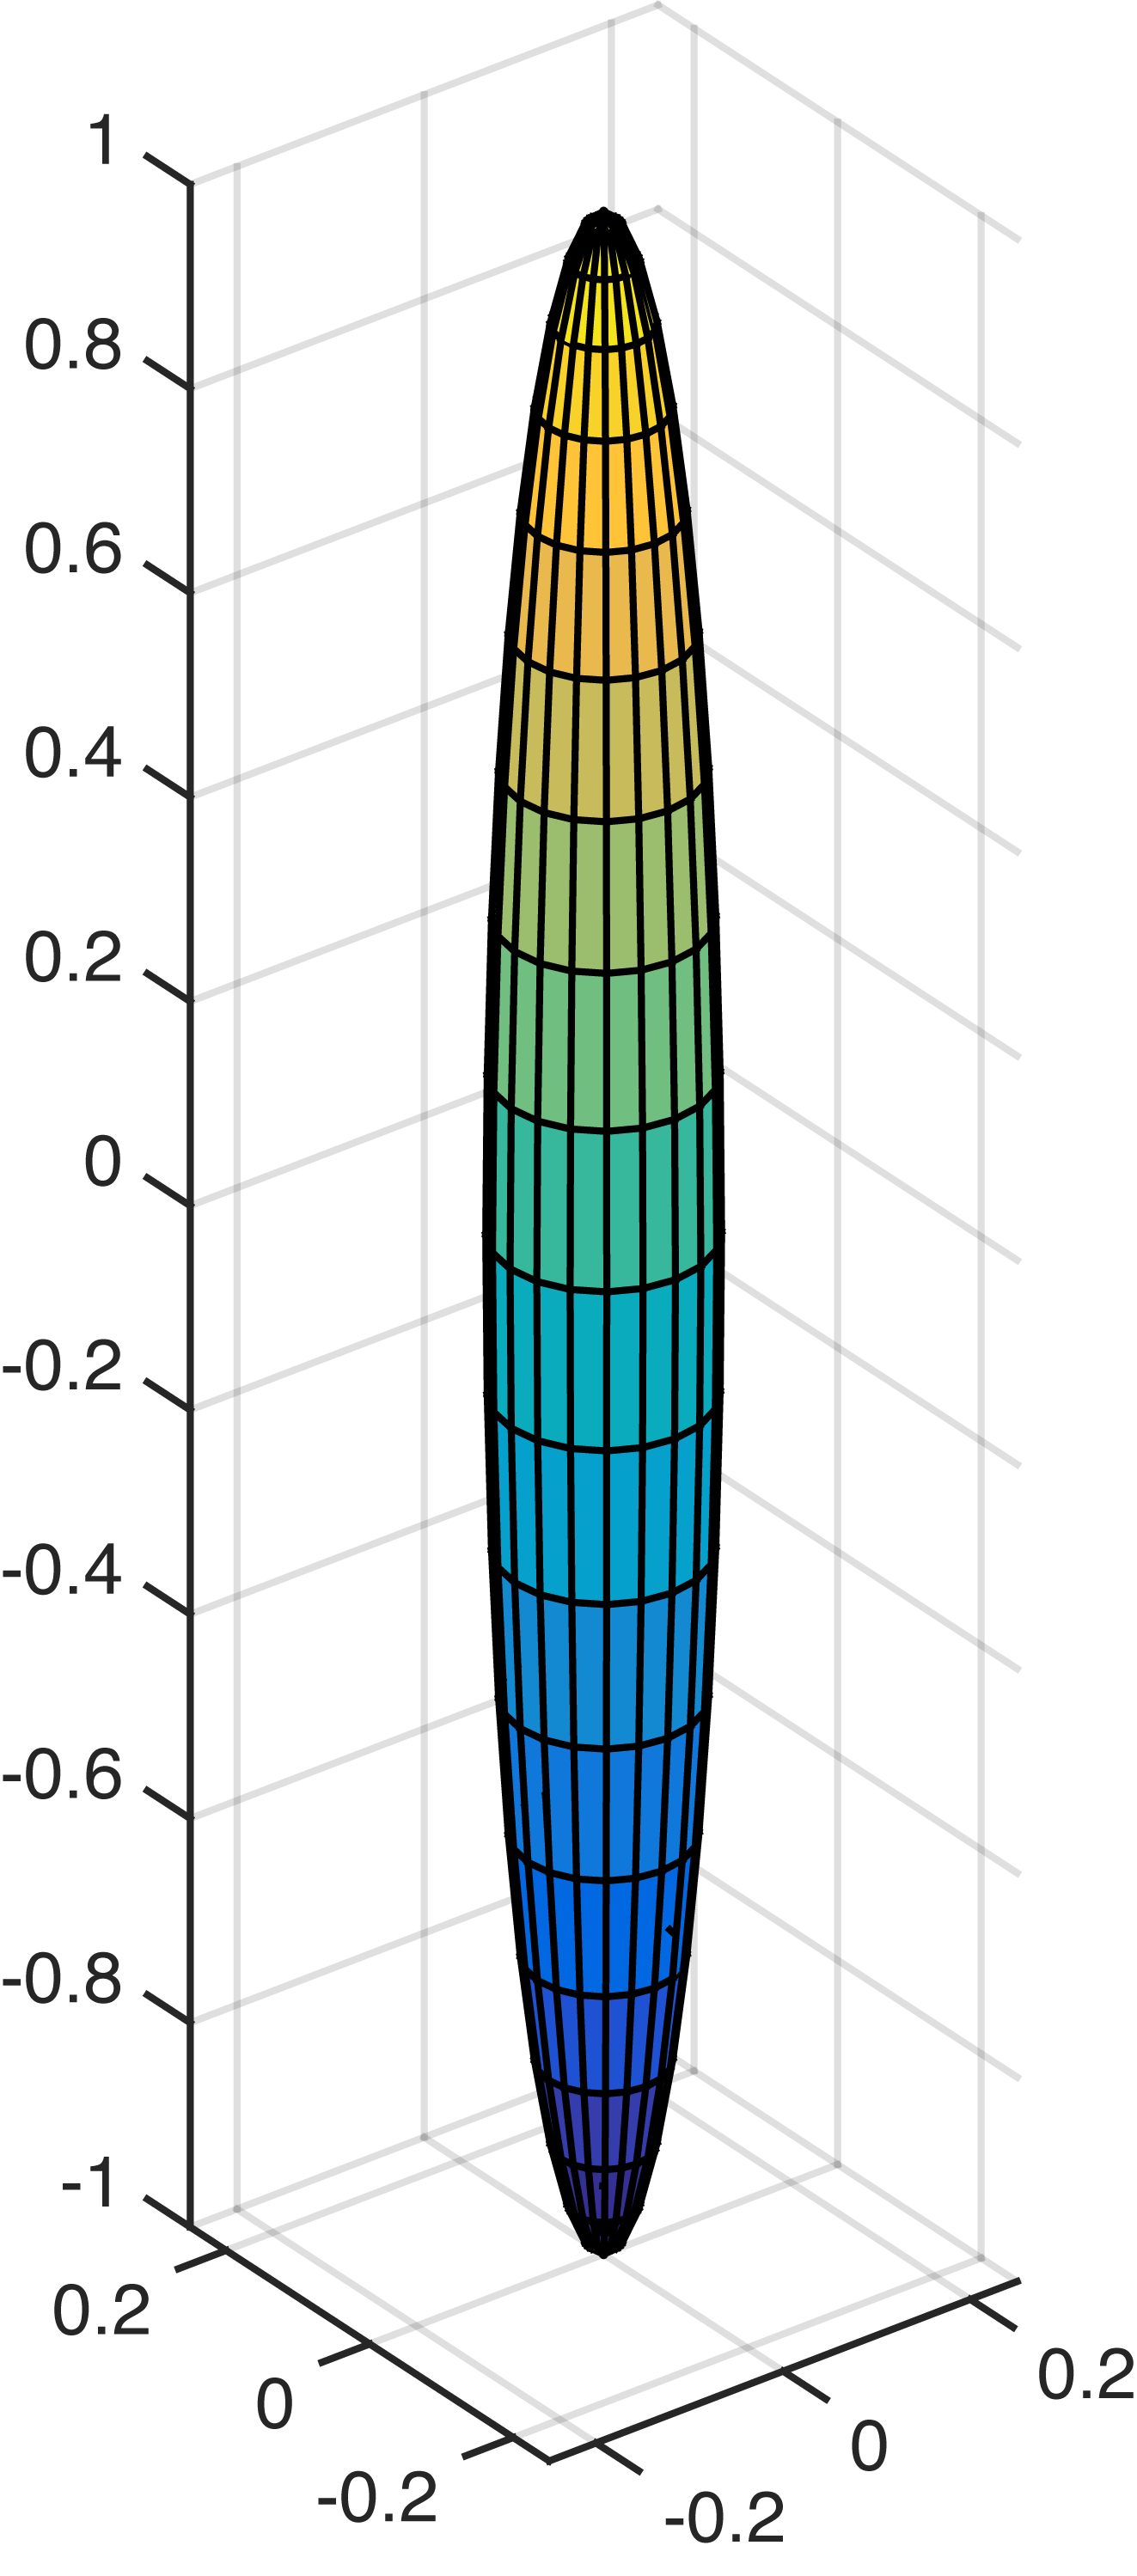
\includegraphics[width=\textwidth]{img/slender/1_10.png}
    \caption{$\epsilon=1/10$}\label{fig:slenderness_1_10}
  \end{subfigure}
  \begin{subfigure}[h]{0.24\textwidth}
    \centering
    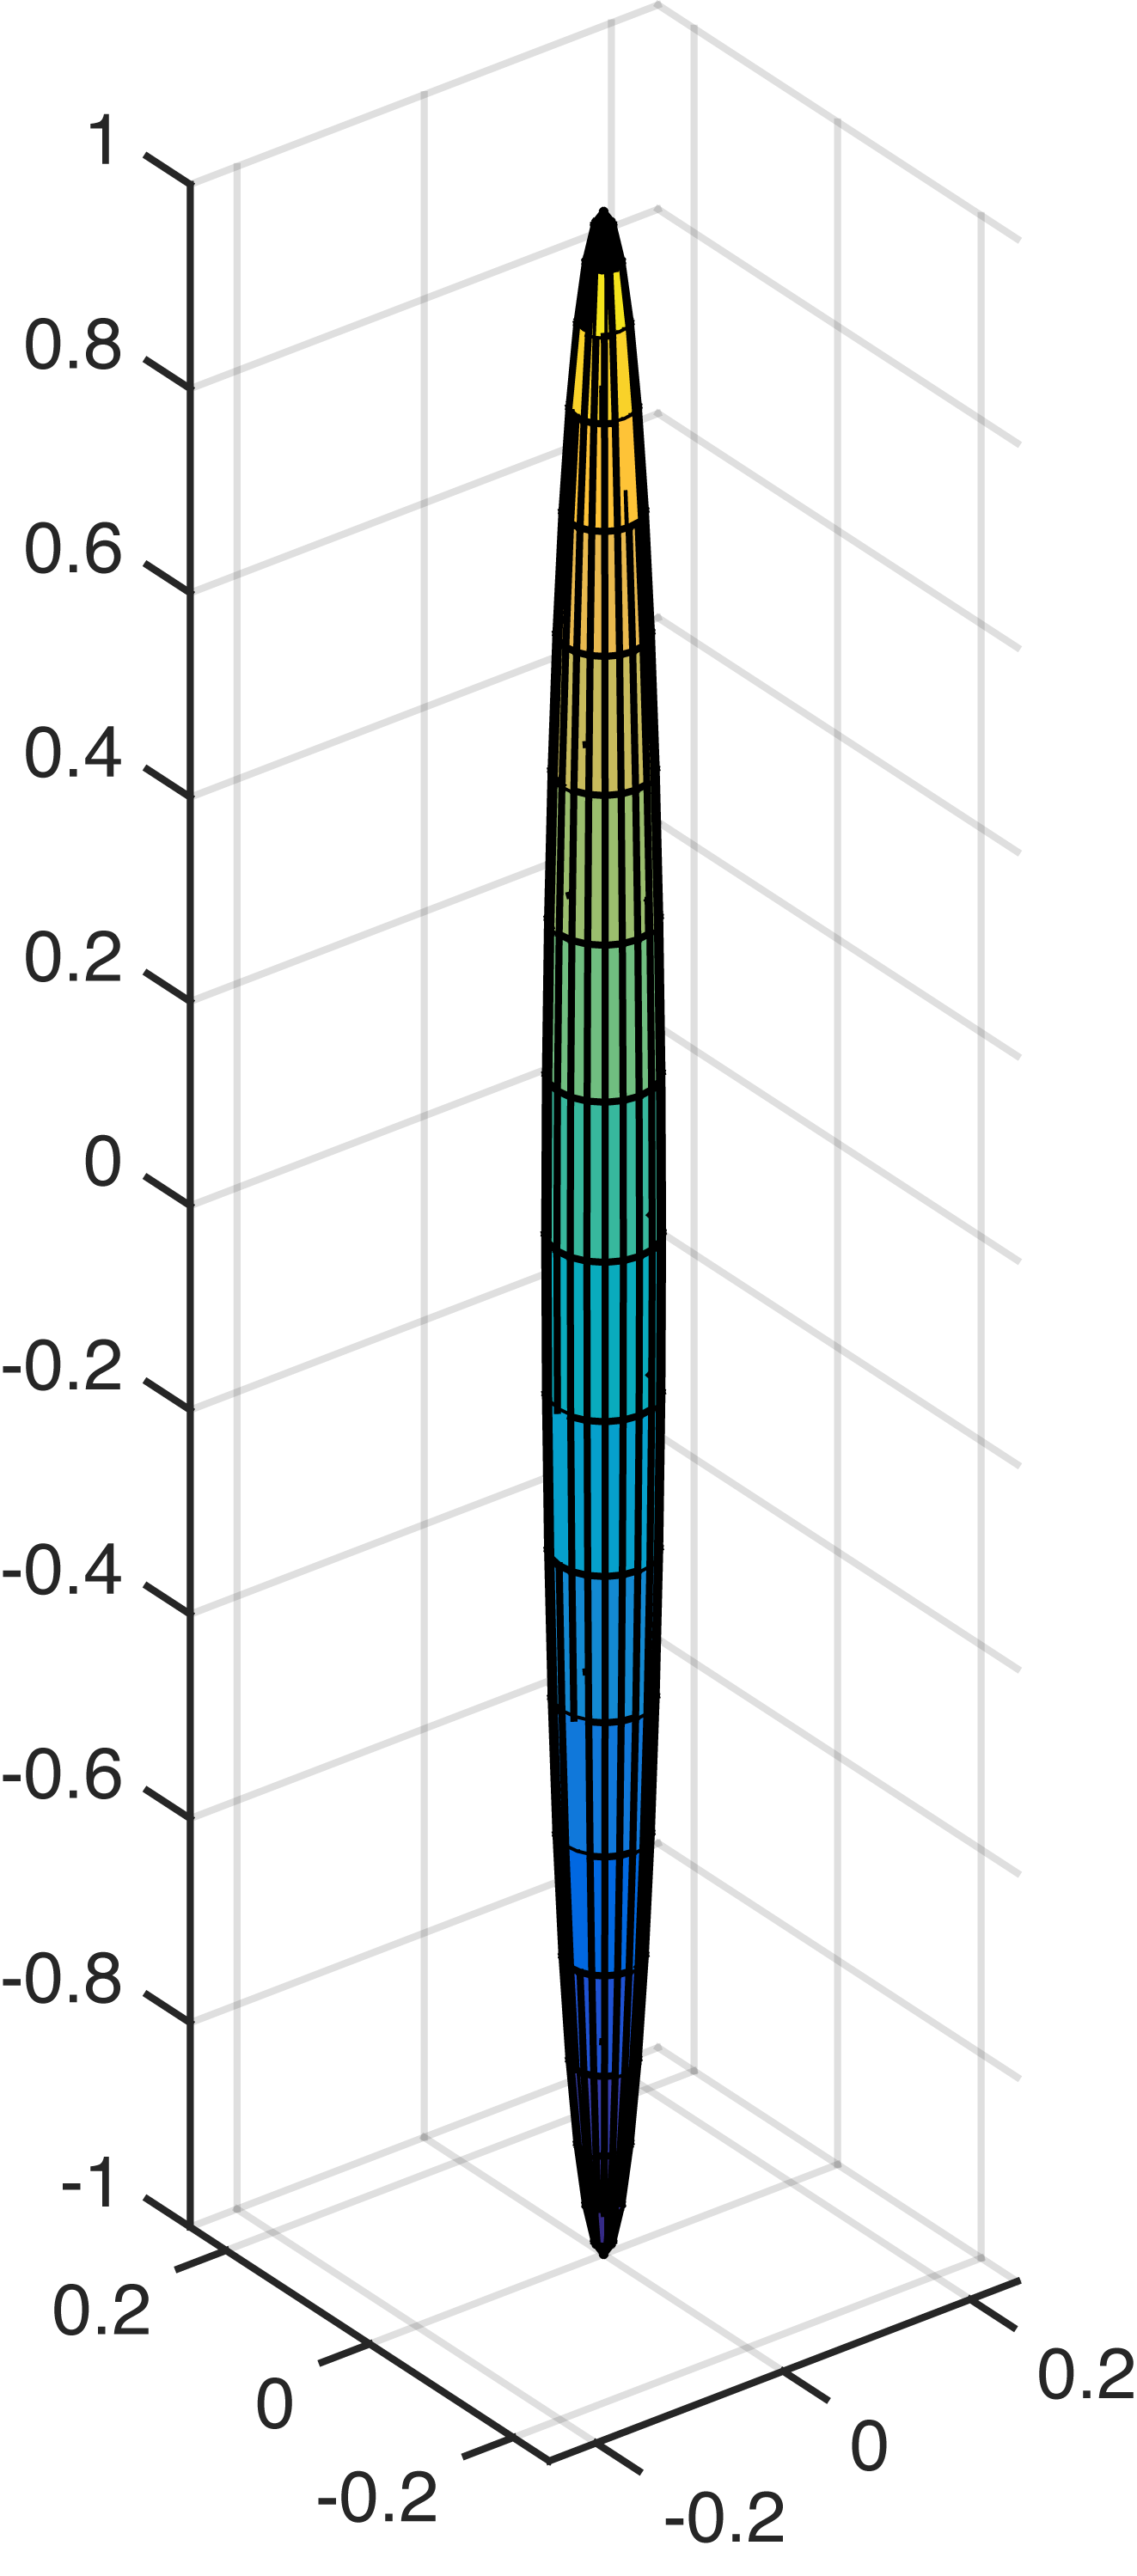
\includegraphics[width=\textwidth]{img/slender/1_20.png}
    \caption{$\epsilon=1/20$}\label{fig:slenderness_1_20}
  \end{subfigure}
  \begin{subfigure}[h]{0.24\textwidth}
    \centering
    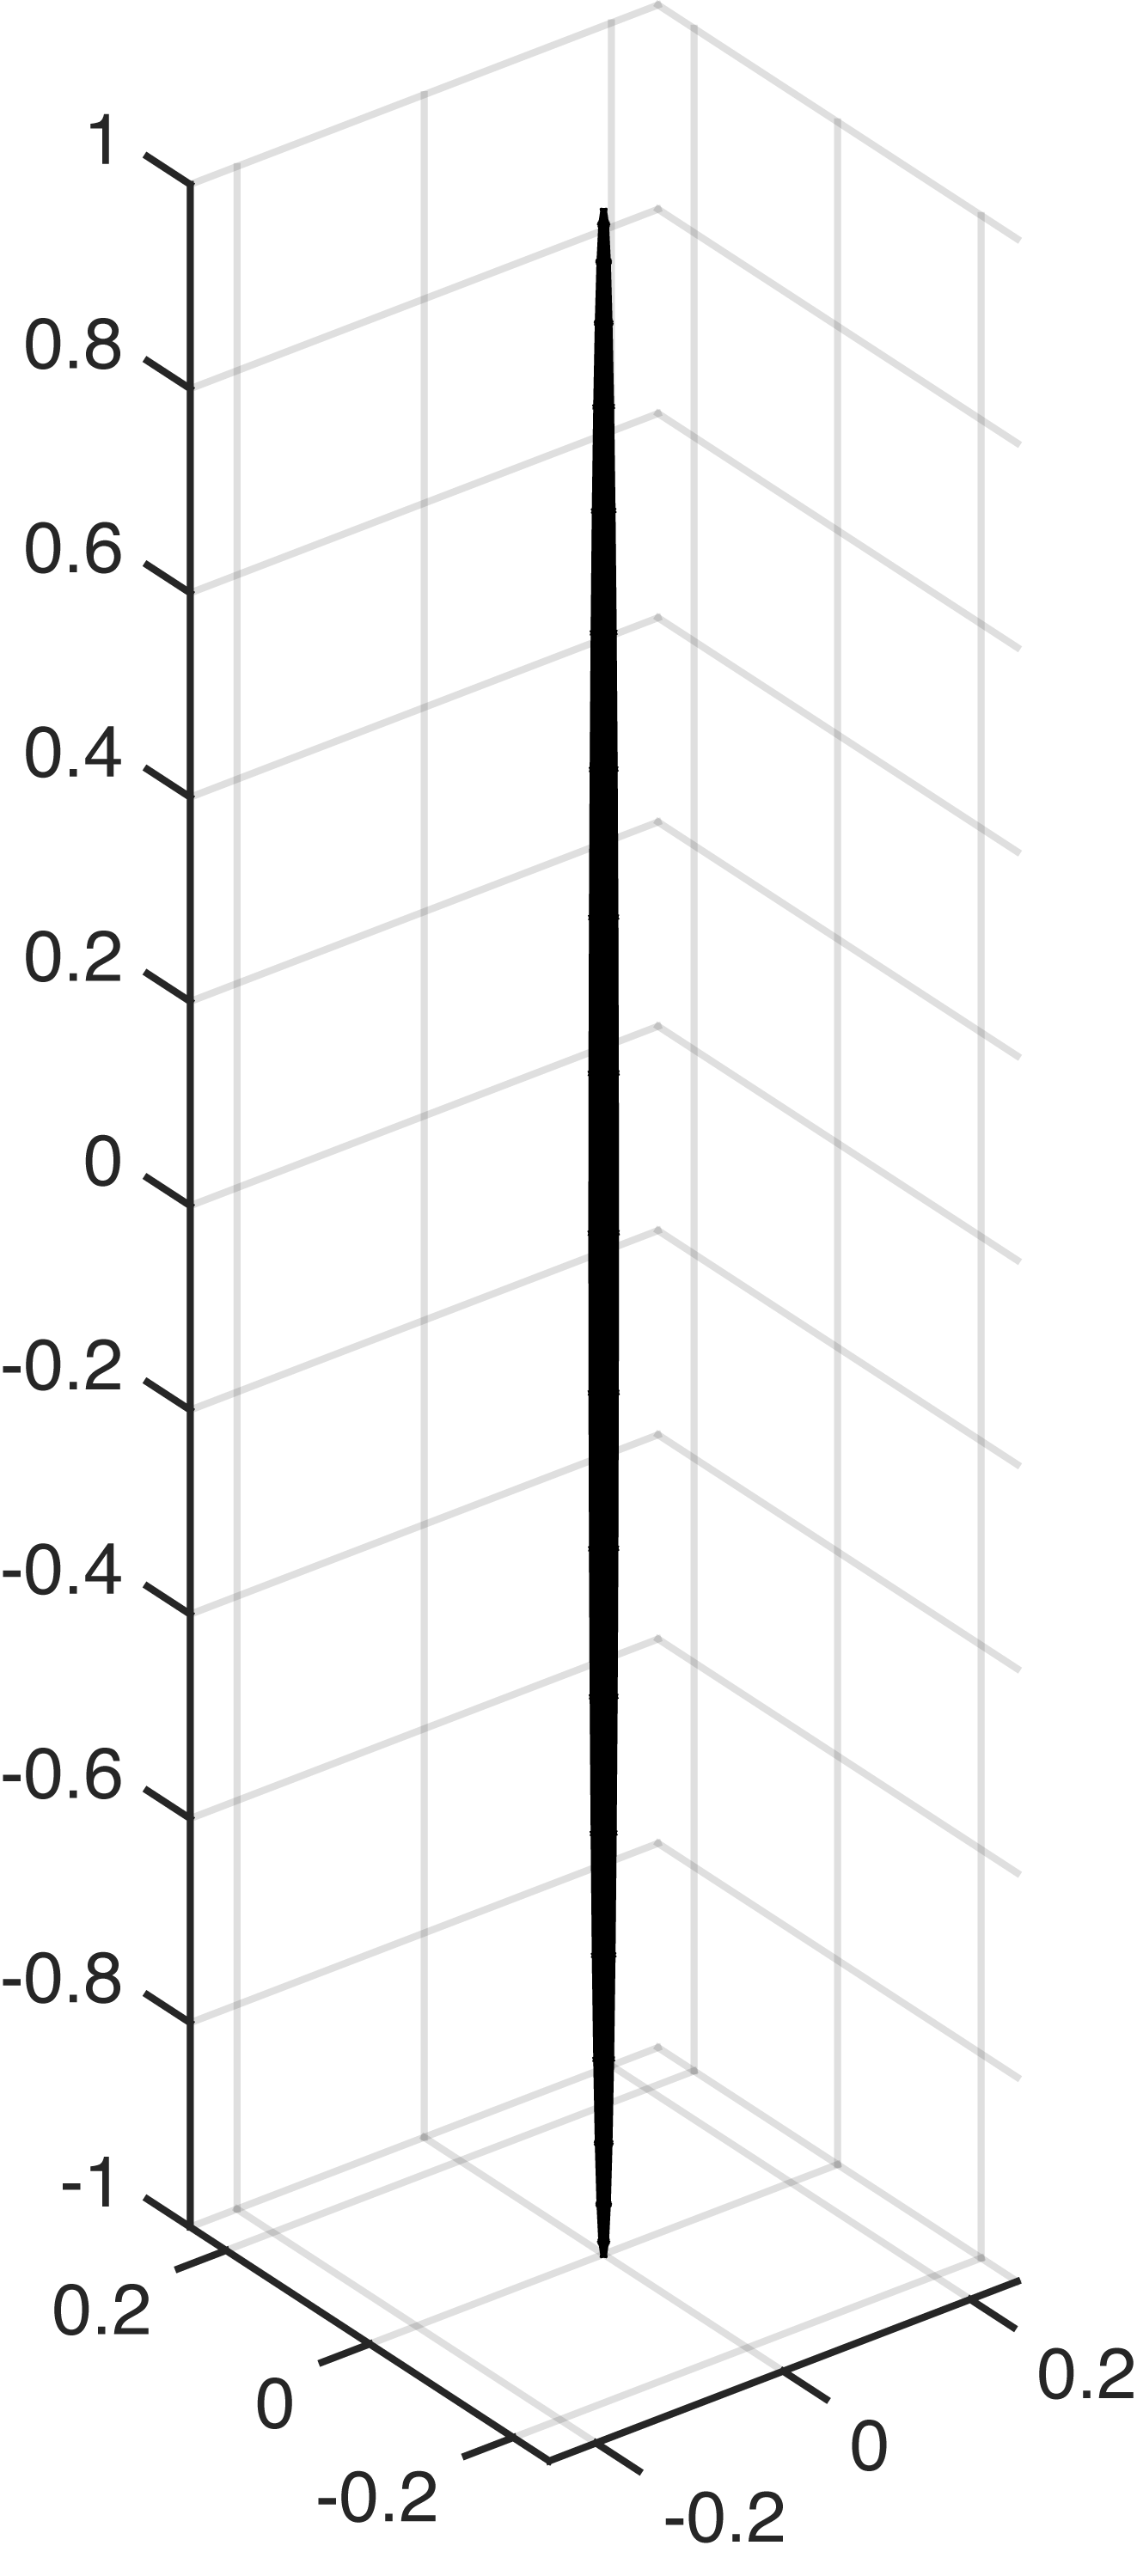
\includegraphics[width=\textwidth]{img/slender/1_100.png}
    \caption{$\epsilon=1/100$}\label{fig:slenderness_1_100}
  \end{subfigure}
  \caption[Illustration of the slenderness parameters.]{Illustration of the slenderness parameters. When $\epsilon$ becomes smaller the shape of the body asymptotically approaches that of an infinitesimal slender fiber.}
  \label{fig:slenderness}
\end{figure}

Our goal is to simulate many slender fibers, but using the 2D boundary integral formulation would be very expensive to solve numerically. As the aspect ratio $1/\epsilon$ of the fiber increases, the requirement of the number of quadrature points also increases in order to accurately resolve the flow field around the fibers. However, for slender bodies a slender body approximation can be used instead. 

The slender body approximation is derived from the boundary integral formulation of the Stokes Eqns.~\eqref{eq:objects_velocity_field}. Using asymptotic analysis the governing surface integrals are reduced to 1D equations along a centerline of the fiber. This is achieved by matching the fluid velocity at a virtual boundary of a slender ellipsoid to the fiber centerline velocity, see Götz,~\cite{Gotz2000}. The accuracy of this approximation is in $O(\epsilon).$ This reduction in dimensionality from 2D boundary integral equations to 1D integral equations is crucial for the ability to include a large number of fibers in the simulations.

The slender body approximation yields a coupled system of 1D integral equations over two fundamental solutions of the Stokes equations, the Stokeslet, Eqn.~\eqref{eq:stokeslet_stokeslet} and the Doublet, Eqn.~\eqref{eq:doublet}. The coupled system relates the forces exerted on the fibers to their velocities and captures the non-local interaction of the fiber with itself (as mediated by the fluid), as well as with any other structures with the fluid, such as other fibers or external boundaries. The system of integral equations is solved using a boundary integral method. Details of the model are given by Tornberg and Gustavsson,~\cite{Tornberg2006}.

\begin{figure}[!htbp]
  \centering
  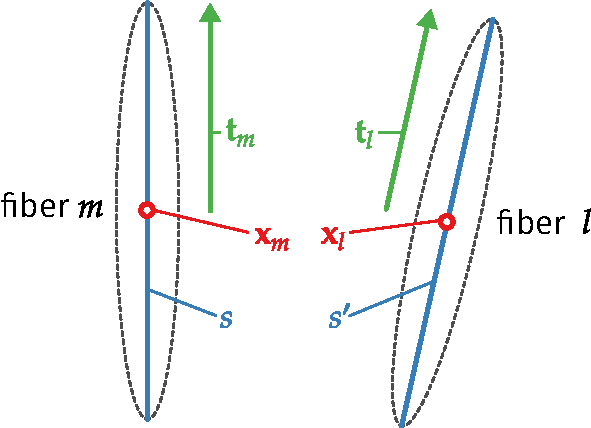
\includegraphics[width=0.5\textwidth]{img/slender.pdf}
  \caption[Slender fiber approximation.]{Slender fiber approximation. Each fiber is described by the center points $\POS_m, \POS_l$ the orientations given by the unit tangent vectors $\ORIENT_m, \ORIENT_l$ and the center line parameterized by $s$ and $s'$. The points on each center line is thus given by $\POS_m(s) = \POS_m + s\ORIENT_m$.}
  \label{fig:slender_fiber}
\end{figure}

Assume that we have $M$ fibers immersed in the fluid. As shown in Fig.~\ref{fig:slender_fiber} each fiber is now defined by its centerline and parameterized by the arc-length, ${s \in [-L,L]}$. For fiber $m$ the coordinates of the centerline are given by \linebreak[4]${\POS_m(s,t) = \POS_m(t) + s\ORIENT_m(t)}$, where $\POS_m$ is the center point and $\ORIENT_m$ the unit tangent vector of the fiber and ${m=1,2,\dots,M}$.

If the fluid exerts a force per unit length, $\mathbf{f}_m$ on fiber $m$, the slender body approximation for the velocity of the centerline of fiber $m$ can be stated in non-dimensional form as
\begin{equation}
  \label{eq:velocity_centerline}
  \begin{aligned}
    d(\dot{\POS}_m + s \dot{\ORIENT}_m) &= \left[ d(\mathbf{I} + \ORIENT_m\ORIENT_m^\top) + 2(\mathbf{I} - \ORIENT_m\ORIENT_m^\top\right]\mathbf{f}_m(s) \\
    &+ (\mathbf{I} + \ORIENT_m\ORIENT_m^\top)\bar{\mathbf{K}}[\mathbf{f}_m](s) + \mathbf{V}_m(s) \text{.}
  \end{aligned}
\end{equation}
Here $d$ is a geometry parameter
\begin{equation}
  \label{eq:geometry_parameter}
  d = -\ln{\epsilon^2e} \text{,}
\end{equation}
and $\bar{\mathbf{K}}[\mathbf{f}_m](s)$ is an integral operator given by
\begin{equation}
  \label{eq:integral_operator}
  \bar{\mathbf{K}}[\mathbf{f}_m](s) = \int_{-1}^{1} \frac{\mathbf{f}(s') - \mathbf{f}(s)}{|s' - s|} \, ds' \text{.}
\end{equation}

The contribution to the velocity of fiber $m$ from the other fibers in the system is accounted for in $\mathbf{V}_m(s)$ as
\begin{equation}
  \label{eq:velocity_contribution}
  \mathbf{V}_m(s) = \sum_{l=1}^M \int_{-1}^{1} \mathbf{G}(\mathbf{R}_{lm}(s,s'))\mathbf{f}_l(s') \, ds' \text{,}
\end{equation}
where $\mathbf{R}_{lm}(s,s') = \POS_m + s\ORIENT_m - (\POS_l + s'\ORIENT_l)$ is the distance between one point on fiber $m$ and one point on fiber $l$ as illustrated in Fig.~\ref{fig:fiber_contribution}.

\begin{figure}[!htbp]
  \centering
  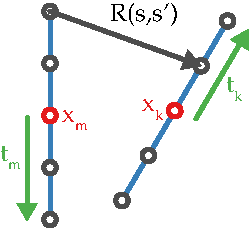
\includegraphics[width=0.3\textwidth]{img/fiber_contribution.pdf}
  \caption[Two interacting fibers with five quadrature points.]{Two fibers with five quadrature points each. The interaction between two fibers is given by the term $\mathbf{V}_m$ and depends solely on the distance between the two. The integral in Eqn.~\eqref{eq:velocity_contribution} can not be evaluated analytically and will be approximated by a quadrature rule.}
  \label{fig:fiber_contribution}
\end{figure}

The Green's function in this case is a linear combination of two fundamental solutions and reads
\begin{equation}
  \label{eq:green_function}
  \mathbf{G}(\mathbf{R}) = \begin{dcases*}
  \mathbf{S}(\mathbf{R}) + \frac{r^2}{2}\mathbf{D}(\mathbf{R}) & if $l \neq m$\\
  0 & if $l = m$
  \end{dcases*}
\end{equation}
with $\mathbf{S}$ and $\mathbf{D}$ as defined in Eqns.~\eqref{eq:stokeslet_stokeslet} and~\eqref{eq:doublet}.

In the non-dimensionalization the half-length of the fiber has been used as a characteristic length, $L_c = L$. This will give use a characteristic velocity and time as
\begin{equation}
  U_C = \frac{d \Delta \rho g V}{4\pi\mu_fL} \text{,} \quad T_C = \frac{2\pi\mu_fL^2}{d \Delta \rho g V} \text{.}
\end{equation}

The unknowns in Eqns.~\eqref{eq:velocity_centerline} are the translational and rotational velocities, $\dot{\POS}_m$ and $\dot{\ORIENT}_m$ and the force distribution along the fiber $\mathbf{f}_m(s)$. To close the formulation of Eqn.~\eqref{eq:velocity_centerline}, we use the additional conditions stating that the integrated force and torque on each fiber must balance the external forces and torques applied to the fibers,
\begin{equation}
	\label{eq:slender_boundary_constraints}
  \mathbf{F}_m = \int_{-1}^{1} \mathbf{f}_m(s) \, ds = \mathbf{F}_g \text{,} \quad \mathbf{T}_m = \int_{-1}^{1} s(\ORIENT_m \times \mathbf{f}_m(s)) \, ds = 0 \text{.}
\end{equation}

For our simulation the external force is just gravity and the external torque is set to zero. Together with this the system is now closed and we can solve our rigid fiber simulation using Eqns.~\eqref{eq:velocity_centerline} and~\eqref{eq:slender_boundary_constraints}.